\chapter{Simulated communications}
\label{cap:annexA}

This annex includes the Python code used for the generation of random communications (Listing \ref{lst:pycom}). The simulated communication activities were inserted in the corresponding collection within the MongoDB database. Note how the \href{https://api.mongodb.com/python/current/tutorial.html}{PyMongo} library was used for this purpose.

The attributes generated in a simulated way and that constitute a communication activity are the following:

\begin{itemize}
\item \textbf{user1} and \textbf{user2}: the users involved in the bidirectional communication activity.
\item \textbf{taskRef}: identification of the task addressed in the communication activity.
\item \textbf{source}: random communication channel.
\item \textbf{duration}: time spent on synchronous communications.
\item \textbf{date}: random date and hour between January and May of 2020.
\item \textbf{project}: project within which the communication is framed.
\end{itemize}

For security reasons, part of the URI used to make the connection to MongoDB Atlas has been omitted. Therefore, the result of the execution will be a set of simulated communications as the ones shown in Figure \ref{fig:coms}.

\newpage
\lstinputlisting[language=Python,style=Python-color,caption={Random communications generator},label=lst:pycom]{./code/communications.py}

\begin{figure}
	\centering
	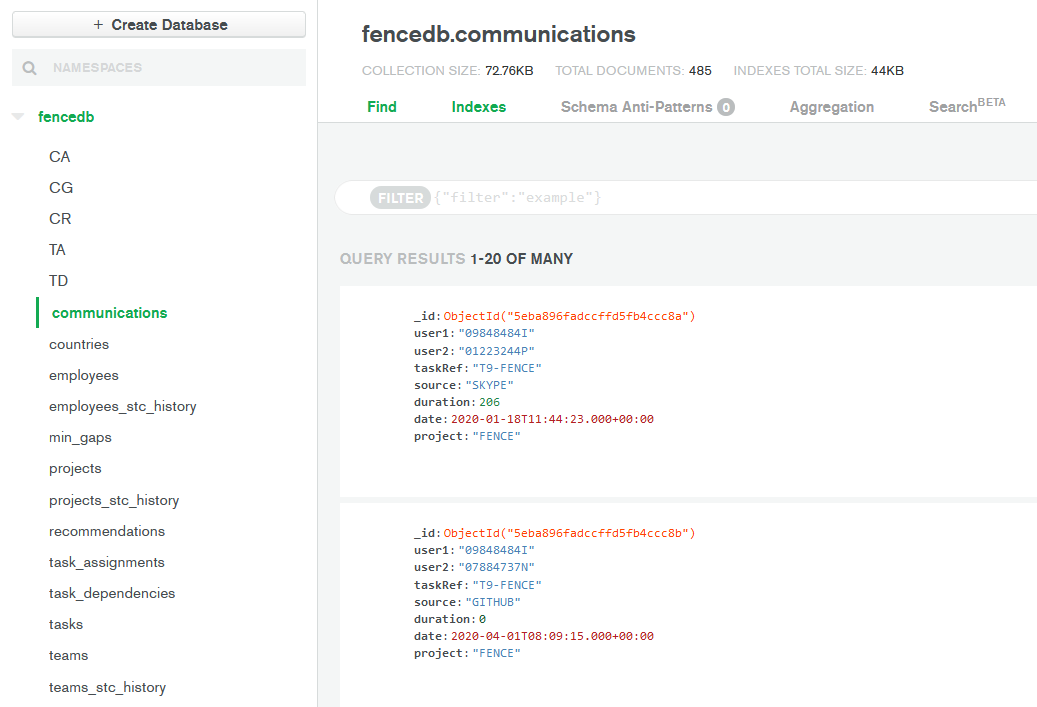
\includegraphics[width=0.95\linewidth]{annex-com}
	\caption[Sample communication activities]{Sample communication activities}
	\label{fig:coms}
\end{figure}

